\documentclass[preprint,12pt,aps,pra,showkeys,amsmath,amssymb,superscriptaddress,floatfix]{revtex4-2}
\usepackage[T1]{fontenc}
\usepackage[utf8]{inputenc}
\usepackage{amsmath,amssymb,amsthm,mathtools,mathrsfs}
\usepackage{microtype,booktabs,enumitem}
\usepackage{xcolor,tikz,etoolbox}
\usepackage[skins,breakable]{tcolorbox}
\usepackage{needspace}
% Keep diagram geometry independent of REVTeX preprint body spacing.
\AtBeginEnvironment{tikzpicture}{\linespread{1}\selectfont}
\usetikzlibrary{arrows.meta,positioning,calc,fit,decorations.pathreplacing}
\usepackage{graphicx}
\usepackage{hyperref}

\definecolor{MMBlue}{RGB}{0,82,155}
\definecolor{MMOrange}{RGB}{200,80,0}
\tikzset{
 mmnode/.style={draw=MMBlue,rounded corners=2pt,fill=MMBlue!4,align=left,execute at begin node={\raggedright},text width=5cm,font=\fontsize{10}{12}\selectfont,inner sep=6pt},
 mmimport/.style={mmnode,draw=black!65,fill=black!4},
 mmcandidate/.style={mmnode,draw=MMOrange,dashed,fill=MMOrange!5},
 mmrejected/.style={mmnode,draw=black,densely dotted,fill=black!8},
 mmproof/.style={->,thick,MMBlue},
 mmflow/.style={->,semithick,black!70},
 mmrepair/.style={->,dashed,thick,MMOrange},
 mmcandidatearrow/.style={->,dashed,semithick,MMOrange},
 mmnote/.style={font=\scriptsize,fill=white,inner sep=2pt,align=center}}

\usepackage[section]{placeins}
\setlength{\emergencystretch}{3em}
\setlist{itemsep=3pt,topsep=4pt}
\newtheorem{theorem}{Theorem}[section]
\newtheorem{proposition}[theorem]{Proposition}
\newtheorem{lemma}[theorem]{Lemma}
\newtheorem{corollary}[theorem]{Corollary}
\theoremstyle{definition}
\newtheorem{definition}[theorem]{Definition}
\newtheorem{example}[theorem]{Example}
\theoremstyle{remark}
\newtheorem{remark}[theorem]{Remark}
% Avoid isolated statement headings and single-line paragraph fragments.
\BeforeBeginEnvironment{theorem}{\Needspace{6\baselineskip}}
\BeforeBeginEnvironment{definition}{\Needspace{5\baselineskip}}
\BeforeBeginEnvironment{proposition}{\Needspace{5\baselineskip}}
\BeforeBeginEnvironment{lemma}{\Needspace{5\baselineskip}}
\BeforeBeginEnvironment{corollary}{\Needspace{5\baselineskip}}
\clubpenalty=5000
\widowpenalty=5000
\newcommand{\R}{\mathbb R}\newcommand{\Z}{\mathbb Z}\newcommand{\N}{\mathbb N}
\newcommand{\Pa}{\operatorname{Pa}}\newcommand{\Desc}{\operatorname{Desc}}
\newcommand{\cl}{\operatorname{cl}}\newcommand{\cost}{\operatorname{cost}}
\newcommand{\status}{\operatorname{status}}
% Faculty cards: a visual rail groups the five faculties within one agent.
% The rail has no arrowhead and does not represent a proof dependency.
\newcommand{\mmfacultybadge}[1]{%
 \node[circle,draw=MMBlue,line width=1pt,fill=white,
 minimum size=7mm,inner sep=0pt,font=\sffamily\small\bfseries,text=MMBlue]
 at ([xshift=15pt,yshift=-15pt]frame.north west) {#1};}
\newcommand{\mmfacultyrail}{%
 \draw[MMBlue!80,line width=1pt]
 ([xshift=15pt,yshift=2pt]frame.north west)--
 ([xshift=15pt,yshift=-2pt]frame.south west);}
\newtcolorbox{mmfacultybox}[2]{enhanced,breakable,
 colback=MMBlue!4,colframe=MMBlue!4,boxrule=0pt,arc=3pt,
 left=39pt,right=9pt,top=7pt,bottom=7pt,
 before skip=2pt,after skip=2pt,
 fontupper=\normalsize\linespread{1.15}\selectfont,
 overlay unbroken={\mmfacultyrail\mmfacultybadge{#1}},
 overlay first={\mmfacultyrail\mmfacultybadge{#1}},
 overlay middle={\mmfacultyrail},overlay last={\mmfacultyrail}}
\newcommand{\mmfaculty}[3]{%
 \begin{mmfacultybox}{#1}{#2}
 {\sffamily\bfseries\color{MMBlue}#2}\par\smallskip #3
 \end{mmfacultybox}}
\newcommand{\agent}[9]{%
 \Needspace{8\baselineskip}
 \subsubsection{#1}
 \noindent\textbf{Object.} #2\par
 \noindent\textbf{Role.} #3\par\smallskip
 \mmfaculty{E}{Ego}{#4}
 \mmfaculty{M}{Memory}{#5}
 \mmfaculty{I}{Intellect}{#6}
 \mmfaculty{S}{Sense}{#7}
 \mmfaculty{A}{Action}{#8}
 \smallskip\noindent #9\par}

\usepackage{longtable,array}
\providecommand{\tightlist}{\setlength{\itemsep}{2pt}\setlength{\parskip}{0pt}}
% Keep short report abstracts with their title instead of REVTeX's optional preprint break.
\makeatletter
\def\frontmatter@abstract@produce{\par\addvspace{\frontmatter@preabstractspace}%
\begingroup\prep@absbox\unvbox\absbox\post@absbox\endgroup
\addvspace{\frontmatter@postabstractspace}}
\makeatother
\newcommand{\field}[2]{\par\smallskip\noindent\textbf{#1.} #2\par}
\newcommand{\reportcaption}[1]{\par\smallskip{\small\noindent #1\par}}


\hypersetup{colorlinks=true,linkcolor=MMBlue,urlcolor=MMBlue,pdftitle={Fundamental Theorem of Arithmetic},pdfauthor={Dibakar Sigdel}}

\begin{document}

\title{Fundamental Theorem of Arithmetic\\[4pt]\large An End-to-End Meta-Math Walkthrough}

\author{Dibakar Sigdel}

\affiliation{Mindverse Computing LLC, Lynnwood, WA 98087, USA}

\date{October 2026}

\begin{abstract}

Existence uses strong induction. Uniqueness uses a different branch:
Bézout gives Euclid's lemma, which matches and cancels prime factors one
at a time. This report presents a complete proof relative to explicit
imports, a dependency graph, versioned node contracts, five-faculty
activities, exact examples, and an illustrative repair. The interactions
are authored explanations, not a transcript of deployed agents or a
proof-assistant certificate.

\end{abstract}

\maketitle

\linespread{1.12}\selectfont

\noindent\textbf{Project NT-02 \quad Report version 1 \quad Number Theory}

\section{Target and import contract}

\begin{theorem}

Every integer \(n\ge2\) can be written as a finite product of primes. If
\(n=p_1\cdots p_r=q_1\cdots q_s\) with all factors prime, then \(r=s\)
and the two lists agree after a permutation, including multiplicities.

\end{theorem}

\subsection{Foundations and permitted imports}

\begin{enumerate}
\def\labelenumi{\arabic{enumi}.}
\item
  A prime is an integer \(p\ge2\) whose only positive divisors are
  \(1,p\). A composite integer \(n\ge2\) has a divisor \(a\) with
  \(1<a<n\), and hence \(n=ab\) with \(1<a,b<n\). Strong induction on
  positive integers is foundational.
\item
  NT-01/N5, v1: for integers \(x,y\) not both zero, there exist integers
  \(u,v\) with \(ux+vy=\gcd(x,y)\). In particular, if a prime \(p\) does
  not divide \(x\), then \(\gcd(p,x)=1\). Unique factorization is not an
  import.
\end{enumerate}

\clearpage\section{Node interaction workflow}

\begin{center}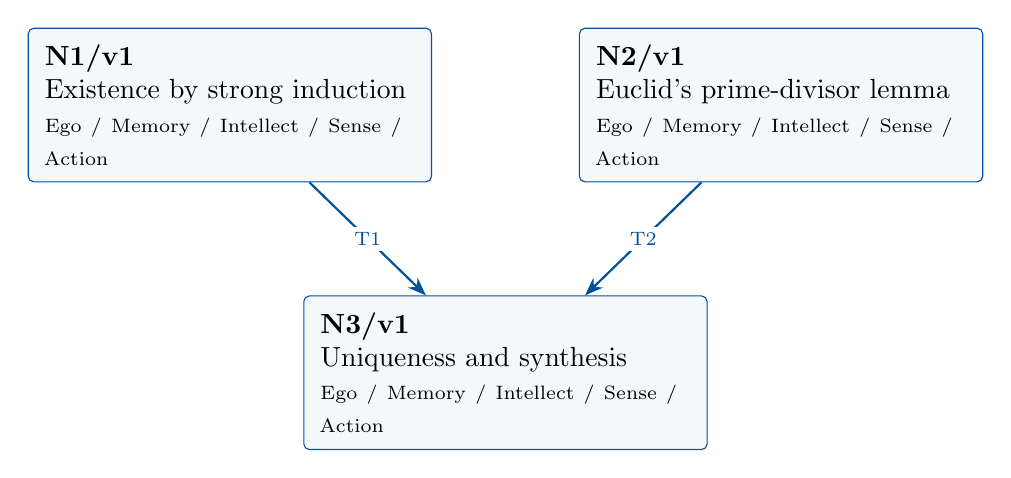
\begin{tikzpicture}[>=Stealth,x=1cm,y=1cm]

\node[mmnode,text width=4.7cm,minimum height=1.35cm] (N1) at (0,0) {\textbf{N1/v1}\\Existence by strong induction\\{\scriptsize Ego / Memory / Intellect / Sense / Action}};

\node[mmnode,text width=4.7cm,minimum height=1.35cm] (N2) at (7,0) {\textbf{N2/v1}\\Euclid's prime-divisor lemma\\{\scriptsize Ego / Memory / Intellect / Sense / Action}};

\node[mmnode,text width=4.7cm,minimum height=1.35cm] (N3) at (3.5,-3.4) {\textbf{N3/v1}\\Uniqueness and synthesis\\{\scriptsize Ego / Memory / Intellect / Sense / Action}};

\draw[mmproof] (N1) to node[mmnote,pos=.5] {T1} (N3);

\draw[mmproof] (N2) to node[mmnote,pos=.5] {T2} (N3);

\end{tikzpicture}\end{center}

\reportcaption{Blue arrows are accepted mathematical dependencies, with exact transfers T1--T2 below. Repair messages are described separately; they are not premises of the proof.}

\subsection{Versioned evidence-transfer ledger}

\begingroup\small\linespread{1.05}\selectfont\renewcommand{\field}[2]{\par\noindent\textbf{#1.} #2\par}

\Needspace{5\baselineskip}\smallskip\noindent\textbf{T1: N1/E1 v1 to N3.3}

\field{Claim}{Every integer \(n\ge2\) has a finite factorization into primes.}

\field{Compatibility}{N1 guarantees a prime product exists; uniqueness compares any two such
products.}

\field{Evidence}{Node N1 activities below and the continuous proof in Section~\ref{sec:proof}.}

\Needspace{5\baselineskip}\smallskip\noindent\textbf{T2: N2/E2 v1 to N3.1}

\field{Claim}{For a prime \(p\), \(p\mid xy\) implies \(p\mid x\) or \(p\mid y\); a
prime dividing a finite nonempty product divides a factor.}

\field{Compatibility}{All compared factors are prime, so finite-product divisibility applies.}

\field{Evidence}{Node N2 activities below and the continuous proof in Section~\ref{sec:proof}.}

\endgroup

\clearpage\section{Agent roles and five-faculty activities}

\subsection{N1/v1: Existence by strong induction}

\field{Object and role}{Build a finite prime product without using uniqueness.}

\field{Inputs}{\(n\ge2\); prime/composite definitions; strong induction.}

\mmfaculty{E}{Ego}{Export existence only, preserving a separate uniqueness obligation.}

\mmfaculty{M}{Memory}{Retain the induction hypothesis for integers \(2\le t<n\).}

\mmfaculty{I}{Intellect}{Split a composite integer into two strictly smaller factors.}

\mmfaculty{S}{Sense}{The factor \(1\) is not prime and cannot provide a decreasing composite
split.}

\mmfaculty{A}{Action}{The base \(n=2\) is prime. Continue with the numbered deductions below,
retaining the exact export.}

\smallskip\noindent\textbf{Numbered mathematical activities}

\begin{enumerate}[label=N1.\arabic*,leftmargin=3.4em]

\item The base \(n=2\) is prime.

\item If \(n\) is prime, use the one-factor product.

\item Otherwise write \(n=ab\) with \(1<a,b<n\); concatenate the two products
supplied by induction.

\end{enumerate}

\field{Export E1/v1}{Every integer \(n\ge2\) has a finite factorization into primes.}

\field{Acceptance gate}{Every integer \(n\ge2\) falls into a prime case or a composite case with
strictly smaller inputs.}

\field{Targeted repair}{If a factor equals \(1\) or \(n\), select a proper divisor before
invoking induction; recheck N3.}

\clearpage

\subsection{N2/v1: Euclid's prime-divisor lemma}

\field{Object and role}{Provide the uniqueness bridge using Bézout, without circular use of
factorization.}

\field{Inputs}{\(p\) prime, \(p\mid xy\); NT-01/N5 Bézout.}

\mmfaculty{E}{Ego}{Restrict the export to prime divisors and record the Bézout import.}

\mmfaculty{M}{Memory}{Retain \(p\nmid x\Rightarrow\gcd(p,x)=1\) and an integer Bézout
certificate.}

\mmfaculty{I}{Intellect}{If the first factor is not divisible by \(p\), transfer divisibility to
the second using a linear combination.}

\mmfaculty{S}{Sense}{The statement fails for composite \(6\) dividing \(2\cdot3\).}

\mmfaculty{A}{Action}{If \(p\mid x\), the conclusion already holds. Continue with the numbered
deductions below, retaining the exact export.}

\smallskip\noindent\textbf{Numbered mathematical activities}

\begin{enumerate}[label=N2.\arabic*,leftmargin=3.4em]

\item If \(p\mid x\), the conclusion already holds.

\item Otherwise write \(up+vx=1\) by Bézout and multiply by \(y\).

\item Since \(p\mid upy\) and \(p\mid vxy\), conclude \(p\mid y\); induct on
the number of factors for a finite product.

\end{enumerate}

\field{Export E2/v1}{For a prime \(p\), \(p\mid xy\) implies \(p\mid x\) or \(p\mid y\); a
prime dividing a finite nonempty product divides a factor.}

\field{Acceptance gate}{Both cases close and the finite-product extension uses induction on its
length.}

\field{Targeted repair}{Restore the prime hypothesis in an overgeneralized candidate and recheck
N3 and every external consumer.}

\clearpage

\subsection{N3/v1: Uniqueness and synthesis}

\field{Object and role}{Match prime factors, cancel in the integers, and join uniqueness to
existence.}

\field{Inputs}{N1/E1, N2/E2; two finite prime products for the same \(n\ge2\).}

\mmfaculty{E}{Ego}{Publish existence and uniqueness together only after multiplicities and
exhaustion are handled.}

\mmfaculty{M}{Memory}{Retain the two prime lists, Euclid's lemma, and integer cancellation by
a nonzero factor.}

\mmfaculty{I}{Intellect}{Remove one matched prime from each list and decrease the remaining
length.}

\mmfaculty{S}{Sense}{A leftover nonempty prime product cannot equal \(1\); repeated primes
must be matched repeatedly.}

\mmfaculty{A}{Action}{Euclid's lemma gives \(p_1\mid q_j\) for some \(j\), so primality forces
\(p_1=q_j\). Continue with the numbered deductions below, retaining the
exact export.}

\smallskip\noindent\textbf{Numbered mathematical activities}

\begin{enumerate}[label=N3.\arabic*,leftmargin=3.4em]

\item Euclid's lemma gives \(p_1\mid q_j\) for some \(j\), so primality forces
\(p_1=q_j\).

\item Permute the second list and cancel the common nonzero integer.

\item Repeat with shorter lists; both must exhaust together, since every prime
is at least \(2\).

\end{enumerate}

\field{Export E3/v1}{Prime factorization exists and its multiset of factors is unique.}

\field{Acceptance gate}{The matching terminates with equal lengths and multiplicities; existence
comes from N1.}

\field{Targeted repair}{If multiplicities are lost, restore lists rather than sets and recheck
the cancellation induction.}

\clearpage\section{Continuous mathematical proof}\label{sec:proof}

\begin{proof}

We first prove existence by strong induction (N1). The integer \(2\) is
prime. For \(n>2\), a prime \(n\) is already a one-factor product.
Otherwise \(n=ab\) for integers \(1<a,b<n\). Applying the induction
hypothesis separately to \(a\) and \(b\) and concatenating the finite
products gives a prime factorization of \(n\).

For uniqueness, prove Euclid's lemma independently (N2). Let \(p\) be
prime and \(p\mid xy\). If \(p\mid x\), there is nothing to prove.
Otherwise the positive common divisors of \(p,x\) consist only of \(1\),
so Bézout (NT-01) gives \(up+vx=1\). Multiplication by \(y\) yields
\[y=upy+vxy.\] Both summands are divisible by \(p\), hence \(p\mid y\).
Induction on the number of factors extends this to any nonempty finite
product.

Now suppose \(p_1\cdots p_r=q_1\cdots q_s\) (N3). The prime \(p_1\)
divides some \(q_j\) by the lemma. Since \(q_j\) is prime and \(p_1>1\),
they are equal. Move \(q_j\) to the front and cancel this nonzero common
factor in the integer equality. Repeating decreases the length of the
first list. If one list were exhausted earlier than the other, an empty
product \(1\) would equal a nonempty product of integers at least \(2\),
a contradiction. Consequently the lists have equal length and matching
factors, with repetitions counted. This proves uniqueness up to
permutation. Together with the independent existence argument it proves
the theorem.

\end{proof}

\section{Worked orchestration}

Existence can split \(360=36\cdot10=(2\cdot3)^2(2\cdot5)\), giving
\[360=2^3 3^2 5.\] For any competing prime product, N2 forces a factor
\(2\). N3 cancels it and compares products for \(180\); repeating gives
\(90\), then \(45\). Two forced cancellations of \(3\) leave \(5\), and
cancelling \(5\) leaves \(1\). An additional factor would make the
remaining product at least \(2\). This trace exhibits the multiplicities
\(3,2,1\); the general proof establishes the claim for all integers.

\subsection{Boundary and hypothesis audit}

\begin{itemize}
\item
  \(n=2\) closes with one factor. The integer \(1\) may be represented
  by an empty product, but is outside the theorem's stated domain.
\item
  Primes cannot be replaced by arbitrary positive divisors:
  \(6\mid2\cdot3\) while \(6\nmid2\) and \(6\nmid3\).
\item
  Integer cancellation here requires only a nonzero factor; it is not
  the modular cancellation rule requiring a unit.
\end{itemize}

\section{Illustrative failure and repair}

This is a deliberately authored teaching trace. A diagnostic asks for
correction; it cannot prove a predecessor by importing its descendant's
conclusion. A revised export must be checked before its consumers are
reused.

\field{Candidate}{N2 proposes \(d\mid xy\Rightarrow d\mid x\) or \(d\mid y\) for arbitrary
\(d>1\).}

\field{Detection}{Sense supplies \(d=6,x=2,y=3\). Memory observes that Bézout with \(x=2\)
gives gcd \(2\), not \(1\).}

\field{Correction}{Intellect restores the prime-divisor contract. Action derives
\(y=upy+vxy\) under \(p\nmid x\).}

\field{Recheck}{Withhold the overgeneralized candidate; recheck N3 and the CRT, Fermat,
and square-factor uses that consume the lemma.}

\field{Publication}{Ego publishes the prime lemma, not the false composite extension. The
original factorization theorem is unchanged.}

\section{Reusable result and provenance}
Reusable exports retain each node's version 1 statement, assumptions, and proof.
The final export is the theorem in Section 1, proved relative to its declared imports.

\smallskip\noindent\textbf{Source record.} Adapted from the original project Markdown:
\par\noindent\nolinkurl{fundamental-theorem-of-arithmetic.md}\par
Typography, workflow conventions, and faculty cards follow the workspace Meta-Math
manuscript. This authored exposition does not claim formal certification.
\end{document}
